%%% SemiClass1.tex --- 
%% Version: $Id: SemiClass1.tex,v 0.0 2012/05/09 03:52:36 tangboyun Exp$
%% Copyright : (c) 2012 Boyun Tang
%% License : BSD-style

\documentclass{standalone}
\usepackage{tikz}
\usetikzlibrary{mindmap,shadows,shapes,positioning,calc,}
\usepackage{graphicx}
\usepackage{times}
\usepackage{xcolor}

\begin{document}

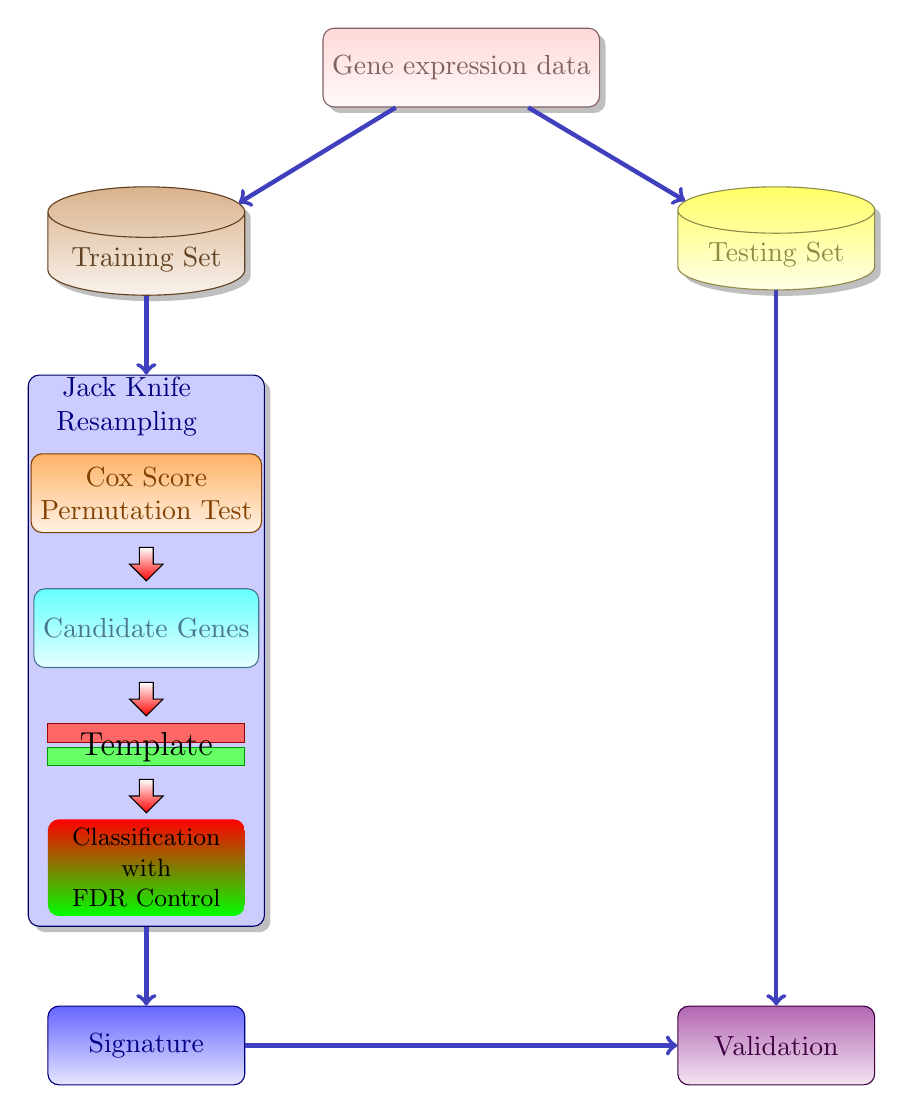
\begin{tikzpicture}[
  every node/.style={minimum width=2.5cm,minimum height=1cm,align=center,},%
  dr/.style={drop shadow},%
  e/.style={->,ultra thick,rounded corners,draw=blue!50!gray},%
  cl/.style={cylinder,aspect=.3,shape border rotate=90,},%
  re/.style={rounded corners,},%
  r/.style={top color= red!60,bottom color= red!10,draw=red!50!black,%
    text=red!50!black,},%
  g/.style={top color= green!60,bottom color= green!10,draw=green!50!black,%
    text=green!50!black,},%
  b/.style={top color= blue!60,bottom color= blue!10,draw=blue!50!black,%
    text=blue!50!black,},%
  br/.style={top color= brown!60,bottom color= brown!10,draw=brown!50!black,%
    text=brown!50!black,},%
  v/.style={top color= violet!60,bottom color= violet!10,draw=violet!50!black,%
    text=violet!50!black,},%
  o/.style={top color= orange!60,bottom color= orange!10,draw=orange!50!black,%
    text=orange!50!black,},%
  ye/.style={top color= yellow!60,bottom color= yellow!10,draw=yellow!50!black,%
    text=yellow!50!black,},%
  p/.style={top color= pink!60,bottom color= pink!10,draw=pink!50!black,%
    text=pink!50!black,},%
  c/.style={top color= cyan!60,bottom color= cyan!10,draw=cyan!50!black,%
    text=cyan!50!black,},%
  a/.style={single arrow,draw,bottom color=red,top color=white,shape border uses incircle,
    shape border rotate=-90,minimum height=.85cm,minimum width=0.1cm,scale=.5}
  ]

  \node (sample) [re,p,dr%
  ] {Gene expression data};

  \node (train) [cl,below=of sample,xshift=-4cm,br,dr%
  ] {Training Set};

  \node (test) [cl,below=of sample,xshift=4cm,ye,dr%
  ] {Testing Set};
  
  \node (frame) [below=of train,re,minimum width=3cm,
  fill=blue!20,minimum height=7cm,
  draw=blue!40!black,dr] {};
  \node (frameword) [text=blue!50!black,
  anchor=north west,yshift=0.1cm] at (frame.north west) {Jack Knife\\Resampling};  
  \node (cox) [below=of frame.north,re,o] {Cox Score\\Permutation Test};

  \node (can) [below=of cox,re,c,yshift=0.3cm] {Candidate Genes};

  \node (tmpp) [below=of can,fill=red!60,draw=red!60!black,yshift=0.3cm,minimum height=0.1cm] {};
  \node (tmpn) [below=of can,fill=green!60,draw=green!60!black,yshift=0cm,minimum height=0.1cm] {};
  \node (tmp) [below=of can,yshift=0.5cm,font=\large] {Template};
  \node (class) [below=of tmp,top color= red,bottom color= green,
  font=\small,yshift=0.6cm,re] {Classification\\with\\FDR Control};
  \node (sig) [below=of frame,re,b] {Signature};
  \path let \p1 = (sig.center), \p2=(test.center) in node (valid) [v,re] at (\x2,\y1) {Validation}; 
  \draw [e] (test) -- (valid);
  \draw [e] (sig) -- (valid);
  \draw [e] (frame) -- (sig);
  \draw [e] (train) -- (frame);
  \draw [e] (sample) -- (train);
  \draw [e] (sample) -- (test);
  \path (cox.south) -- (can.north) node [midway,a] {};
  \path (can) -- (tmpp) node [midway,a] {};
  \path (tmpn) -- (class) node [midway,a] {};
\end{tikzpicture}
\end{document}

%%% Local Variables: 
%%% TeX-master: "../../LaTeX/"
%%% End: 
